\documentclass[aspectratio=169]{beamer}
\usepackage[utf8]{luainputenc}
\usepackage[TS1,T1]{fontenc}
\usepackage{babel}
\usetheme[pagenum,navbar,ddc]{tud}
\usepackage{xcolor}
\usepackage{listings}
\usepackage{tikz}
\usepackage{mathtools}
\usepackage[labelformat=empty,font=scriptsize]{caption}
\usepackage{multicol}
\usepackage{marvosym}
\usepackage{wasysym}
\usepackage{tikz}
\usepackage[pscoord]{eso-pic}% The zero point of the coordinate systemis the lower left corner of the page (the default).

\newcommand{\placetextbox}[3]{% \placetextbox{<horizontal pos>}{<vertical pos>}{<stuff>}
	\setbox0=\hbox{#3}% Put <stuff> in a box
	\AddToShipoutPictureFG*{% Add <stuff> to current page foreground
		\put(\LenToUnit{#1\paperwidth},\LenToUnit{#2\paperheight}){\vtop{{\null}\makebox[0pt][c]{#3}}}%
	}%
}%

\newcommand{\theory}[1]{\text{Th}\left( #1 \right)}
\newcommand{\lang}[1]{\text{L(}#1{)}}

\title{Decidability \protect\\\mdseries of Logical Theories\strut}
\subtitle{Proseminar Theoretical Computer Science}
\author{Lucas Waclawczyk}

\newcommand*\inmm[1]{\pgfmathsetmacro\inmmwert{#1 / 1mm}\inmmwert}
\makeatletter
\newcommand*\inpt[1]{\setlength\@tempdima{#1}\the\@tempdima}
\makeatother

\AtBeginSection[]{\partpage{\usebeamertemplate***{part page}}}
\begin{document}
	\mode<presentation>{\setbeamertemplate{tud background}[image/shaded]{Seminarraum.jpg}{0.7}}
	\maketitle
	
	\mode<presentation>{\setbeamertemplate{page number in footline}[frame][text and total]}
	\frame{\frametitle{Inhalt}\tableofcontents}
	
	\section{Basics}
	\begin{frame}{First-Order Logic}
		\[
			\forall q \: \exists p \: \forall x \: \forall y \:\: \Bigg[
				R_{1}(p, q) \wedge \Big(
					\neg \big(
						R_{1}(x, 1) \wedge R_{1}(y, 1)
					\big) \vee R_{2}(x, y, p)
				\Big)
			\Bigg]
		\]
		
		\vspace{.25cm}
		\only<2->{\noindent\rule[.25ex]{\textwidth}{.3pt}}
		\vspace{.25cm}
		\begin{tabular}{p{.5\linewidth}p{.5\linewidth}}
			\visible<2->{
				Formulas consist of:
				\begin{itemize}
					\visible<2->{\item Quantifiers: $ \forall, \: \exists $}
					\visible<3->{\item Variables: $ p, q, x, y, \dots $}
					\visible<4->{\item Boolean operators: $ \wedge, \vee, \neg $}
					\visible<5->{\item Relation symbols: $ R_{1}, R_{2}, \dots $}
					\visible<6->{\item Special characters: $ [, ], (, ) $}
				\end{itemize}
			}
			&
			\visible<7->{
				Simplified here:
				\begin{itemize}
					\visible<7->{\item mostly "sentences"}
					\visible<8->{\item only prenex normal form}
				\end{itemize}
			}
		\end{tabular}
	\end{frame}

	\begin{frame}{First-Order Logic}
		\only<1-4>{
			\[
				\forall q \: \exists p \: \forall x \: \forall y \:\: \Bigg[
					R_{1}(p, q) \wedge \Big(
						\neg \big(
							R_{1}(x, 1) \wedge R_{1}(y, 1)
						\big) \vee R_{2}(x, y, p)
					\Big)
				\Bigg]
			\]
		}
		\vspace{-.3cm}
		
		\only<2>{\centering$ \stackrel{!}{=} \:\:$ "There are infinitely many prime numbers."}
		
		\only<4->{
			\[
				\only<4>{= \quad} \forall q \: \exists p \: \forall x, y \:\: [p>q \wedge (x, y > 1 \rightarrow xy \neq p)]
			\]
		}
		
		\only<5>{
			\vspace{-.3cm}
			\[	
				\text{vs. } \: [(x + x = y) \: \vee \: (x \geq y) ]
			\]
		}
		
		\only<6>{
			\vspace{-.3cm}
			\[	
				\text{vs. } \: \forall y \: \exists x \: \: [\neg (xx \neq y)]
			\]
		}
	
		\only<7>{\centering$ = \:\:$ "There are infinitely many prime numbers."}
		
		\vspace{.25cm}
		\only<3->{\noindent\rule[.25ex]{\textwidth}{.3pt}}
		\vspace{.25cm}
		\begin{tabular}{p{.5\linewidth}p{.5\linewidth}}
			\only<3->{ 
				\begin{itemize}
					\only<3->{\item \emph{universe} $ \mathcal{U} $
						\begin{itemize}
							\item possible values for variables
							\item here $ \mathbb{N} $
						\end{itemize}
					}
				\only<1-4>{\end{itemize}&}
				\only<4>{\begin{itemize}}
					\only<4->{\item \emph{model} $ \mathcal{M} $
						\begin{itemize}
							\item universe + assignment of relations
							\item here $ (\mathbb{N},\: >_{2},\: (\times \neq)_{3}) $
						\end{itemize}
					\end{itemize}
					}
			}
			\only<5->{
				&
				\begin{itemize}
					\only<5->{\item \emph{language} $ \lang{\mathcal{M}} $
						\begin{itemize}
							\item sentences that make sense in $ \mathcal{M} $
							\item here $ \lang{\mathbb{N},\: >_{2},\: (\times \neq)_{3}} $
						\end{itemize}
					}
					\only<6->{\item \emph{theory} $ \theory{\mathcal{M}} $
						\begin{itemize}
							\item true sentences formed with $ \mathcal{M} $
							\item here $ \theory{\mathbb{N},\: >_{2},\: (\times \neq)_{3}} $
						\end{itemize}
					}
				\end{itemize}
			}
		\end{tabular}
	\end{frame}

	\begin{frame}{What Is Decidability?}
		\begin{itemize}
			\item here: for logic (there is a more general definition)
			\item let $ \mathcal{M} $ be a model, $ \varphi \in \lang{\mathcal{M}} $
		\end{itemize}
		
		\[
			\theory{\mathcal{M}} \text{ decidable } \coloneqq
		\]\[
			\text{ there is an algorithm that decides whether } \varphi \text{ is true in } \mathcal{M} 
		\]
	\end{frame}

	\section{$ \theory{\mathbb{N}, +} $ -- A Decidable Theory}
	\begin{frame}{Theorem 1}
		\begin{theorem}
			$ \theory{\mathbb{N}, +} $ is decidable.
		\end{theorem}
		
		\vspace{1cm}
		\uncover<2->{i.e., there is an algorithm that can decide, whether a sentence $ \varphi \in \lang{\mathbb{N}, +} $ is true or false.}
	\end{frame}

	\begin{frame}{Review: Automata}
		\begin{figure}
			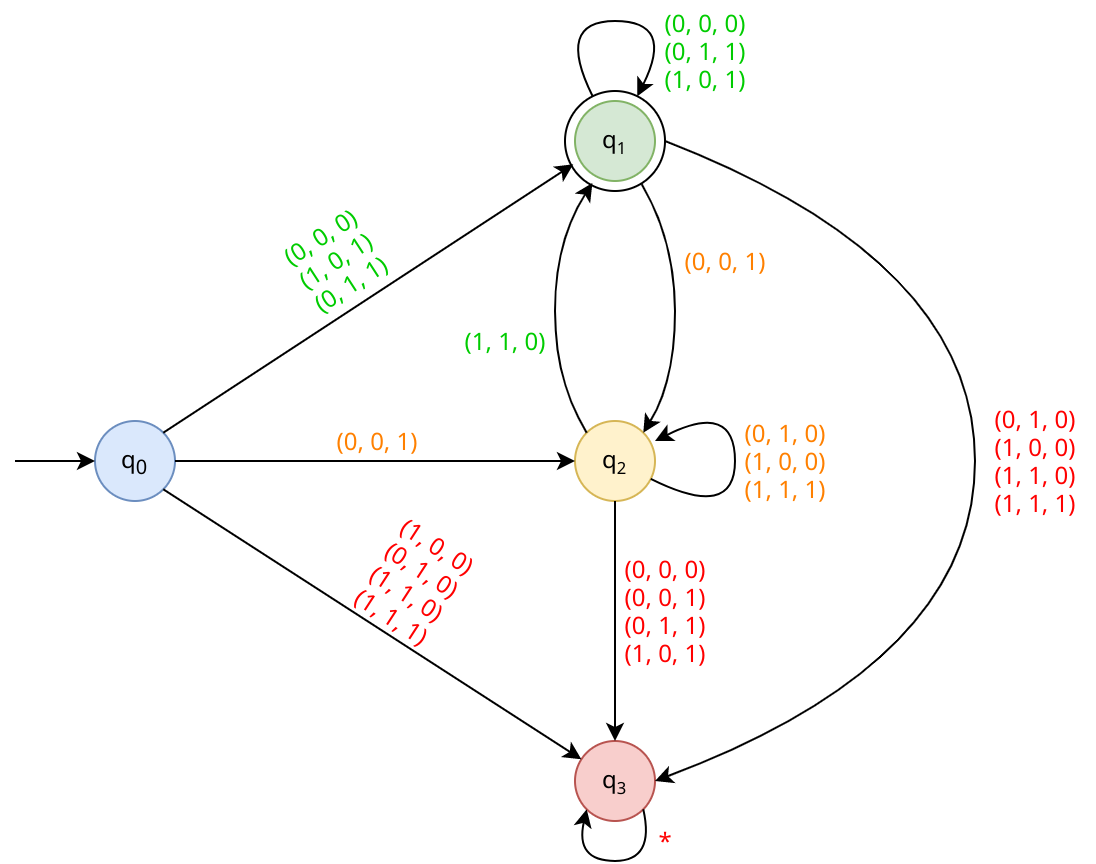
\includegraphics[width=.55\linewidth]{addition}
			\caption{Example automaton that accepts all correct binary additions}
		\end{figure}
	\end{frame}

	\begin{frame}{Proof of Theorem 1}
		\textbf{Idea: } Construct an automaton that accepts an (almost) empty input iff the given sentence is true.
		\vspace{.5cm}
		
		Let $ i \in \mathbb{N} \setminus \{0\} $ and define $ \Sigma_{i} \coloneqq \{0, 1\}^{i} $ and $ \Sigma_{0} \coloneqq \{()\} $. 
		
		An example for a word in $ \Sigma_{3} $:
		\[
			\begin{pmatrix}
				0\\
				1\\
				1
			\end{pmatrix}
			\begin{pmatrix}
				0\\
				0\\
				1
			\end{pmatrix}
			\begin{pmatrix}
				1\\
				1\\
				0
			\end{pmatrix}
			\quad \sim \quad
			\begin{pmatrix}
				1\\
				5\\
				6
			\end{pmatrix}
		\]
	\end{frame}

	\begin{frame}{Proof of Theorem 1}
		\visible<1->{
			Now, let 
			\begin{itemize}
				\setlength{\itemsep}{1em}
				\item $ i \in \{0, \dots, l\} $
				\item $ \varphi = Q_{1} x_{1} \dots Q_{l} x_{l} \: [\psi(x_{1}, \dots, x_{l})] \in \lang{\mathbb{N}, +} $ \hspace{.3cm} where $ Q_{1}, \dots, Q_{l} \in \{\forall, \exists\} $
				\visible<2->{
					\item $ \varphi_{i} \coloneqq Q_{i+1} x_{i+1} \dots Q_{l} x_{l} \: [\psi(x_{1}, \dots, x_{l})] $
					\begin{itemize}
						\item[$ \Rightarrow $] $ \varphi_{0} = \varphi $
						\item[$ \Rightarrow $] $ \varphi_{l} \coloneqq \psi $
					\end{itemize}
				}
				\visible<3->{
					\item $ \varphi_{i}(a_{1}, \dots, a_{i}) \coloneqq Q_{i+1} x_{i+1} \dots Q_{l} x_{l} \: [\psi(a_{1}, \dots, a_{i}, x_{i+1}, \dots, x_{l})]$
				}
			\end{itemize}
		}
	
		\vspace{.3cm}
		\visible<4->{
			\[
				\Longrightarrow \qquad
				\varphi_{l} \:\: \text{ is only a Boolean expression.}
			\]
		}
	\end{frame}

	\begin{frame}{Proof of Theorem 1}
		Construct an automaton $ A_{l} $ that behaves like $ \varphi_{l} = \psi $, meaning $ A_{l} $ accepts exactly the tuples $ (a_{1}, \dots, a_{l}) \in \mathbb{N}^{l} $\: for which $ \varphi_{l}(a_{1}, \dots, a_{l}) $ is true:
		\vspace{.3cm}
		
		\begin{itemize}
			\item Take one addition automaton for each addition term in $ \varphi_{l} $
			\item Combine them:
				\begin{itemize}
					\item automaton product for $ \wedge $
					\item automaton union for $ \vee $
					\item automaton complement for $ \neg $
				\end{itemize}
				in a way that they behave like $ \varphi_{l} $.
		\end{itemize}
		\vspace{.3cm}
		
		\visible<3->{
			\textbf{Important:} There is an algorithm that constructs $ A_{l} $ from $ \varphi_{l} $
		}
	\end{frame}

	\begin{frame}{Proof of Theorem 1}
		\only<1,3->{
			If $ Q_{i} = \exists $, construct automaton $ A_{i} $ from $ A_{i+1} $ by
			\begin{itemize}
				\item copying $ A_{i+1} $
				\item adding a new start state and one state for each character in $ \Sigma_{i} $
				\item making $ A_{i} $ guess the right $ a_{i+1} $ non-deterministically
			\end{itemize}
		}
	
		\only<2>{
			\begin{figure}
				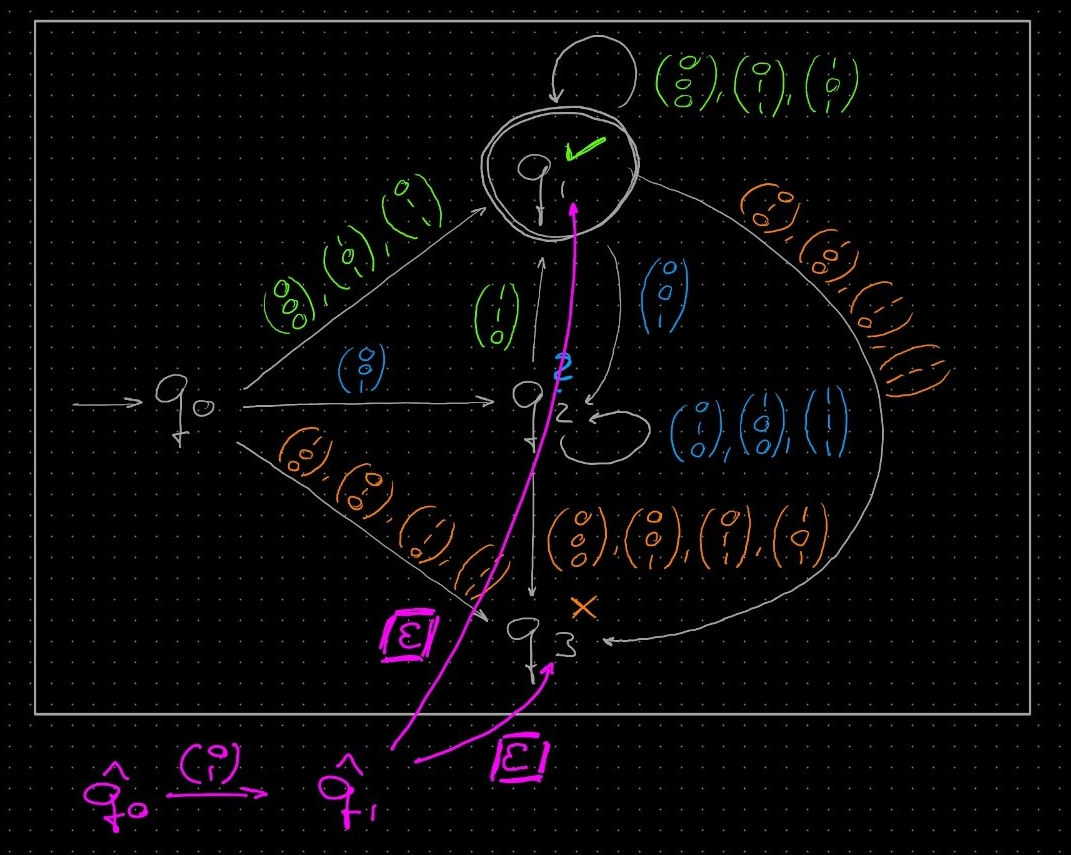
\includegraphics[width=.55\linewidth]{non-det_guessing}
				\caption{Example construction of non-deterministic guessing}
			\end{figure}
		}
	
		\vspace{.3cm}
		\visible<3->{
			If else $ Q_{i} = \forall $, use complementation twice ($ \forall x_{i} \varphi_{i+1} = \neg \exists x_{i} \neg \varphi_{i+1} $)
		}
		
		\vspace{.3cm}
		\visible<4->{
			$ \Longrightarrow \qquad A_{i} $ accepts input $ (a_{1}, \dots, a_{i}) \in \mathbb{N}^{i} \quad \Leftrightarrow \quad \varphi_{i} $ is true
		}
	
		\vspace{.3cm}
		\visible<5->{
			$ \Longrightarrow \qquad A_{0} $ accepts input $ () \quad \Leftrightarrow \quad \varphi_{0} = \varphi $ is true
		}
	
		\vspace{.3cm}
		\visible<6->{
			Let the algorithm return "$ \varphi \in \theory{\mathbb{N}, +} $" $ \quad \Leftrightarrow \quad A_{0} $ accepts input $ () $
		}
	\end{frame}

	\section{$ \theory{\mathbb{N}, +, \times} $ -- An Undecidable Theory}
	\begin{frame}{Theorem 2}
		$ \theory{\mathbb{N}, +, \times} $ is undecidable
		
		\vspace{1cm}
		\uncover<2->{i.e., there is no algorithm that can decide, whether a sentence $ \varphi \in \lang{\mathbb{N}, +} $ is true or false.}
	\end{frame}

	\begin{frame}{Turing Machines}
		\begin{figure}
			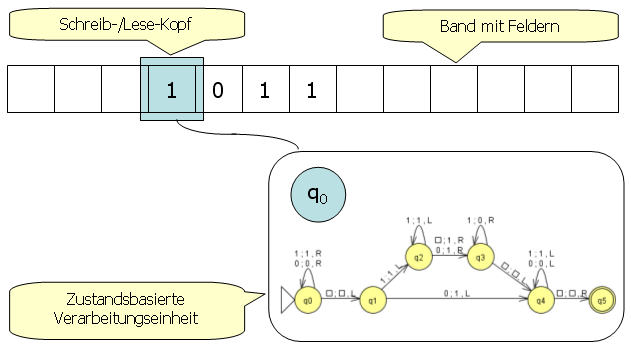
\includegraphics[width=.7\linewidth]{turing_machine}
			\caption{Example turing machine\\source: \hyperlink{ref:turing}{[2]}}
		\end{figure}
	\end{frame}

	\begin{frame}{Proof Idea for Theorem 2}
		\begin{itemize}
			\visible<1->{
				\item The word problem for Turing machines is undecidable.
			}
			\visible<2->{
			\item There is a mapping reduction that translates
				\begin{itemize}
					\item a Turing machine $ M $ and a string $ w $
					\visible<3->{
						\item to a formula $ \varphi_{M, w} \in \theory{\mathbb{N}, +, \times} $ that contains only one free variable $ x $, such that
					}
					\visible<4->{
						\item $ \varphi_{M, w} $ is true $ \: \Leftrightarrow \: x $ is a (suitably encoded) computation history of $ M $ with which $ M $ accepts $ w $
					}
				\end{itemize}
			}
		\end{itemize}
	
		\vspace{.3cm}
		\visible<5->{
			Assume $ \theory{\mathbb{N}, +, \times} $ is decidable.
		
			$ \Longrightarrow \quad $ The formulas $ \exists x \varphi_{M, w} \in \theory{\mathbb{N}, +, \times} $ are decidable.
		}
	
		\visible<6->{
			$ \Longrightarrow \quad $ The word problem for Turing machines is decidable.
		}
	
		\visible<7->{
			$ \Longrightarrow \quad $ \Lightning
		}
	\end{frame}

	\begin{frame}{Thinking further...}
		Assumptions:
		\begin{itemize}
			\item [A$ _{1} $] Proofs can be checked by a machine.
			\item [A$ _{2} $] Provable statements are true.
		\end{itemize}
		
		\vspace{.3cm}
		\visible<2->{
			Lemmas:
			\begin{enumerate}
				\item \label{item1} The provable statements of $ \theory{\mathbb{N}, +, \times} $ are Turing recognizable.
				\\\textbf{Proof idea:} Just try all possible (suitably encoded) proofs.
				\visible<3->{
					\item There is a true statement in $ \theory{\mathbb{N}, +, \times} $ that is not provable.
					\\\textbf{Proof idea:} Contradiction to Theorem 2 by using \ref{item1}. 
				}
			\end{enumerate}
		}
	\end{frame}

	\section{Gödel's Incompleteness Theorem}
	\begin{frame}{A True, Unprovable Statement}
		We can construct a true statement in $ \theory{\mathbb{N}, +, \times} $, that is not provable.
		
		\visible<2->{
			\vspace{.3cm}
			\textbf{Construction:}
			Let $ M $ be a Turing machine that operates as follows.
			\begin{itemize}
				\item Delete the input
				\item Look for proof of $ \neg \exists x [\varphi_{M, 0}] \in \theory{\mathbb{N}, +, \times} $
				\item Accept on proof, reject if no proof can be found
			\end{itemize}
		}
		
		\vspace{.3cm}
		\visible<3->{
			$ \Longrightarrow \quad \neg \exists x [\varphi_{M, 0}] $ is the wanted statement.
		}
	\end{frame}

	\begin{frame}{Gödel's Method}
		\begin{itemize}
			\visible<1->{
				\item Construct the statement "This statement cannot be proved by the axioms."
			}
			\visible<2->{
				\item Argue against just adding this statement to the axiom.
			}
		\end{itemize}
	
		\vspace{.3cm}
		\visible<3->{
			$ \Longrightarrow \qquad $ Incompleteness \: \smiley
		}
	\end{frame}

	\section{Conclusion}
	\begin{frame}{Conclusion}
		$ \Longrightarrow \qquad $ There are (very simple) indecidable logical theories.
		
		\vspace{.3cm}
		\visible<2->{
			$ \Longrightarrow \qquad $ Mathematics cannot be mechanized.
		}
		
		\vspace{.3cm}
		\visible<3->{
			$ \Longrightarrow \qquad $ No sound logical system can be complete.
		}
	\end{frame}

	\section{References}
	\begin{frame}{References}
		\begin{itemize}
			\item [{[1]}] Martin Alessandro - Own work, CC BY-SA 4.0, \url{https://commons.wikimedia.org/w/index.php?curid=75082873} \label{ref:automata}
			\item [{[2]}] \url{https://www.inf-schule.de/grenzen/berechenbarkeit/turingmaschine/station_turingmaschine} \label{ref:turing}
			\item [{[3]}] Michael Sipser: Introduction to the Theory of Computation. Thomson Course Technology, 2006
			\item [{[4]}] \url{https://www.youtube.com/watch?v=O4ndIDcDSGc}
			\item [{[5]}] Prof. Dr. Franz Baader: Skript Theoretische Informatik und Logik (Sommersemester 2020), TU Dresden
		\end{itemize}
	\end{frame}
\end{document}
